\section{Routing e Sicurezza}
\subsection{Routing Statico}
Il routing statico, anche denominato come instradamento statico, è un metodo che sfrutta percorsi prefissati dall’amministratore di rete. In questa maniera si può configurare un'intera rete molto velocemente, anche se con alcuni svantaggi. Infatti, il routing statico, avendo gli indirizzi fissi nelle varie macchine della rete, non è efficiente nella risoluzione di possibili errori. 

Il grande problema, infatti, si ha nel direzionare il pacchetto nella rete, se il percorso previsto per il pacchetto ha un errore al suo interno il traffico non viene ridirezionato e attende finché il percorso non sia stato riparato o finché l'amministratore di rete non abbia definito una nuova rotta. 

Nonostante ciò, però, il routing statico è ancora molto utilizzato e permette a piccole sottoreti interconnesse di lavorare al meglio e con pochi sforzi di gestione.

\subsubsection*{Configurazione computer con IP statici}
Per assegnare degli indirizzi IP in maniera statica ai dispositivi in una rete bastano 4 step, vediamone un esempio concreto svolto su CISCO packet tracer:

\begin{enumerate}
    \item Per prima cosa aprire la finestra relativa al dispositivo in questione (in questo caso un PC)\par
    \begin{sfigure}
        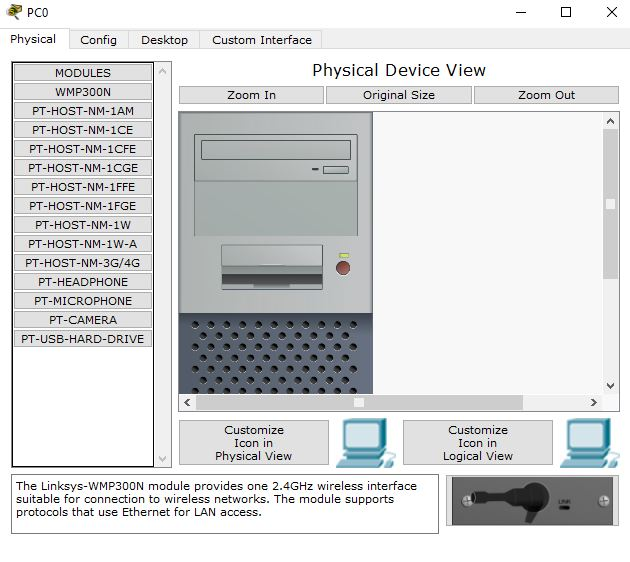
\includegraphics[width=0.6\linewidth]{images/07.routing-sicurezza/01.open-pc.jpg}
    \end{sfigure}
    \item Entrare nel Desktop del pc tramite il menu sovrastante\par
    \begin{sfigure}
        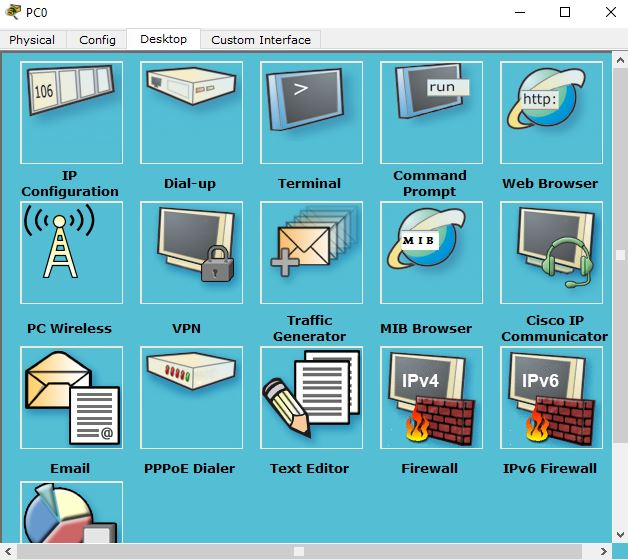
\includegraphics[width=0.6\linewidth]{images/07.routing-sicurezza/02.desktop-tab.jpg}
    \end{sfigure}
    \item Entrare nel menu della configurazione IP tramite l’icona presente nel desktop\par
    \begin{sfigure}
        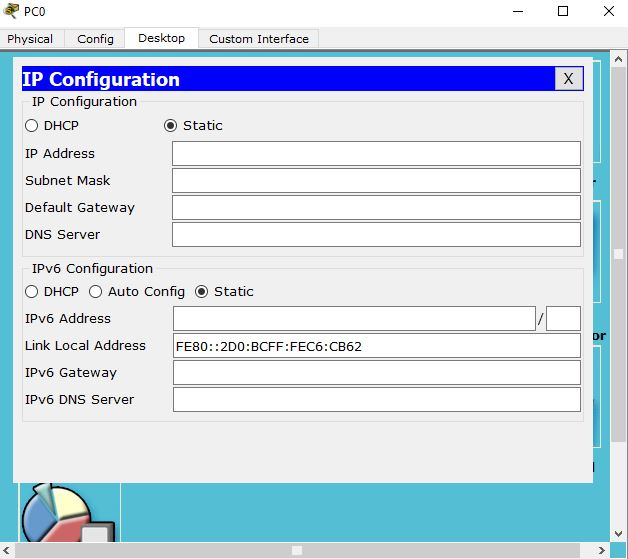
\includegraphics[width=0.6\linewidth]{images/07.routing-sicurezza/03.ip-config.jpg}
    \end{sfigure}
    \item In conclusione, inserire i dati riguardante gli indirizzi IP all’interno degli appositi come nell’esempio sotto riportato\par
    \begin{sfigure}
        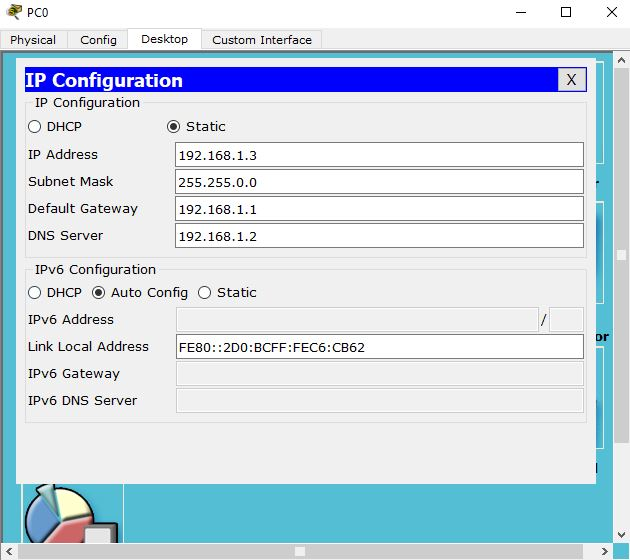
\includegraphics[width=0.6\linewidth]{images/07.routing-sicurezza/04.ip-config-complete.jpg}
    \end{sfigure}
\end{enumerate}

\subsubsection*{IP Route}
Il comando ip route è essenziale per la comunicazione tra reti a routing statico, dato che permette di creare rotte statiche e di conseguenza, instaurare il collegamento tra sottoreti. La sintassi del comando è molto semplice come vedremo a breve

Ecco come aggiungere una rotta tra router:

\begin{cmds}[Router]{Configuration mode}{cmd:ip-route-example}{Aggiungere una rotta statica nel router che indirizza i pacchetti destinati alla \textcolor{Highlight1}{rete specificata} verso l'\textcolor{Highlight2}{indirizzo IP o l'interfaccia} designata }
    \$ ip route \textcolor{Highlight1}{192.168.1.0 255.255.255.0} \textcolor{Highlight2}{172.16.100.1}
\end{cmds}

\subsection{VLAN}
Con il termine VLAN (Virtual Local Area Network) si intende la suddivisione di una rete locale, definita da uno switch, in più reti virtuali non comunicanti tra di loro ma appartenenti alla stessa infrastruttura fisica.

Per procedere alla suddivisione di una rete locale in più VLAN è necessario programmare lo switch a cui è associata la rete, quindi accedere alla console e digitare i seguenti comandi:

\begin{cmds}[Switch]{Configuration mode}{cmd:create-vlan}{Creare una VLAN in uno switch con \textcolor{Highlight1}{id} e \textcolor{Highlight2}{nome} arbitrario tuttavia la VLAN con ID 1 è utilizzata come default quindi convenzionalmente si utilizza la cifra delle decine (10, 20, ...)}
    \$ vlan \textcolor{Highlight1}{10}\\
    \$ name \textcolor{Highlight2}{sinistra}\\
    \$ vlan \textcolor{Highlight1}{20}\\
    \$ name \textcolor{Highlight2}{destra}
\end{cmds}

Una volta definite le VLAN si può procedere ad assegnare ad ogni rete virtuale le porte dello switch, suppondendo che lo switch abbia 24 porte in totali:

\begin{cmds}{Configuration mode}{cmd:setup-vlan-ports}{Configurazione delle porte dello switch modificando l'intero \textcolor{Highlight1}{range} di porte e assegnandole ad una \textcolor{Highlight2}{determinata VLAN}}
    \$ interface range \textcolor{Highlight1}{Fa 0/5-14}\\
    \$ switchport mode access\\
    \$ switchport access \textcolor{Highlight2}{vlan 10}\\
    \$ interface range \textcolor{Highlight1}{Fa 0/15-24}\\
    \$ switchport mode access\\
    \$ switchport access \textcolor{Highlight2}{vlan 20}
\end{cmds}

Un dettaglio importante di cui tenere conto quando si progettano le VLAN è quello di lasciare alcune porte non assegnate, così da poter definire eventuali porte di tronco. Una porta di tronco è una porta dello switch collegata ad un dispositivo esterno alle VLAN (come un router) e serve per permettere la comunicazione tra VLAN e i dispositivi collegati a quella porta.

Definizione di una porta di tronco:

\begin{cmds}[Switch]{Interfaccia esterna}{cmd:trunk-port}{Configurazione dell'interfaccia di tronco}
    \$ switchport mode trunk\\
    \$ switchport trunk allowed vlan
\end{cmds}

\subsection{VPN}
Una VPN (Virtual Private Network) è una rete privata virtuale che utilizza una rete pubblica per collegare tra loro terminali remoti, come se fossero sulla stessa rete locale (LAN) criptandone il traffico internet e di conseguenza proteggendo anche l’identità online delle parti comunicanti. Per fare in modo che ciò avvenga, viene sfruttato l’instradamento dei pacchetti di dati tramite il protocollo IP per il trasporto su scala geografica: questo permette, di fatto, di realizzare una LAN virtuale e privata ma del tutto equivalente ad un’infrastruttura fisica di rete dedicata.

Ne esistono due tipologie:

\begin{itemize}
    \item Accesso Remoto: permette di mascherare l’indirizzo IP con il quale si accede alla rete, permette di connettersi da remoto a un server su una rete privata per il tramite della rete Internet. Rappresenta un collegamento tra un PC client VPN e il server a cui si vuole avere accesso remoto.
    \item Site to Site: connette tra loro due o più reti private in varie località collocate in vari Paesi del mondo in una unica rete privata, ogni rete dovrà avere ovviamente il suo router dedicato che fungerà da nodo nella VPN per instradare pacchetti verso i destinatari seguendo il modello Client-Server. Utilizza canali non sicuri come il web, per effettuare una connessione sicura creano un ponte virtuale (tunneling) che unisce le varie posizioni per fare sì che accedano alla rete internet e mantengono una connessione sicura tra le reti permettendo la condivisione di informazioni in modo trasparente per tutta la rete.
    
    Esistono due tipi sottoclassi di VPN site-to-site

    \begin{itemize}
            \item Intranet: quando si uniscono più sedi della stessa azienda; 
            \item Extranet: quando si uniscono aziende e/o uffici esterni all’organizzazione.
    \end{itemize}
\end{itemize}

Al loro interno le VPN possono essere ulteriormente classificate in base al loro livello di affidabilità in:

\begin{itemize}
    \item TRUSTED: L’ISP (Internet Service Provider) garantisce la creazione di una serie di percorsi dotati di precise caratteristiche di sicurezza, assegnando un determinato indirizzo IP fisso e applicando una corretta politica di sicurezza delle informazioni.
    
    Chi utilizza le Trusted VPN si collega al primo nodo di rete dell’operatore, successivamente il pacchetto di dati viene inoltrato dal mittente al destinatario (nel quale è implementato l’MPLS) aggiungendo una label che lo identifica che verrà poi rimossa dall’ISP del destinatario che consegnerà poi il pacchetto.

    La trusted VPN presenta molti vantaggi per quanto riguarda sicurezza, affidabilità e qualità del servizio, perché viene tutto gestito dal provider e dal fornitore che si occuoperanno di garantire sicurezza e di fornire i percorsi ottimali per ogni evenienza, quindi il cliente non ha responsabilità, gli algoritmi che compongono queste VPN sono interni allla rete e quindi la fault recovery è molto più veloce e meno soggetta a manifestarsi ed infine viene creata un’unica LAN logica grazie al piano di indirizzamento IP che è lo stesso del cliente. Gli unici svantaggi di questo tipo di VPN sono i costi elevati e la rigidità del servizio.

    \item SECURE: Questo tipo di VPN, attraverso protocolli di crittografia, garantisce la creazione di un tunnel tra i nodi della rete privata. I dati che viaggiano all’interno del tunnel risultano pertanto inaccessibili a tentativi d’intercettazione;
    
    Una volta scelte, implementate e usate, alcune tecniche possono fornire comunicazioni sicure su reti non affidabili. Le tecnologie delle Secure VPN dovrebbero essere utilizzate come security overlay attraverso infrastrutture di rete dedicate.

    Il vantaggio principale delle Secure VPN è che i tunnel VPN essendo creati utilizzando protocolli di cifratura e sicurezza come IPsec, TSL/SSL, PPTP (Point to Point Tunneling Protocol) o SSH e che questi protocolli sono utilizzati da entrambi i nodi di una VPN. Di conseguenza, se un hacker riuscisse a intercettare i pacchetti di un traffico di rete, vi troverebbe dentro solo dati illeggibili.

    \item HYBRID: Come specificato dal nome si tratta di una particolare tipologia di rete privata mista. Si applica nei casi in cui una azienda dotata di una Trusted VPN avesse bisogno anche di una Secure VPN. Con una VPN ibrida si garantisce così una buona sicurezza ed un certo livello di qualità del servizio dei circuiti di tunneling.
    
    Un hybrid VPN mette insieme MPLS, protocolli di sicurezza internet o VPN IPsec, anche se questi due tipi di VPN sono usati in maniera separata per siti diversi. In ogni caso, è possibile usarli entrambi per lo stesso sito. Questo può essere fatto con l’intenzione di usare il VPN IPsec come backup per il VPN MPLS.

    Le hybrid VPNs sono usate dalle compagnie perché gli MPLS non sarebbero la scelta più appropriata per il loro sito. Ci sono numerosi vantaggi nell’utilizzo degli MPLS comporta al posto della connessione internet pubblica, tuttavia, i costi sono elevati. Inoltre, usando un hybrid VPN si può avere accesso al sito centrale da un sito a distanza. Questo tipo di VPN è piuttosto costoso anche se molto flessibile.
\end{itemize}

\subsubsection{Protocolli}
Di seguito verranno elencati e spiegati i vari protocolli delle VPN:

\begin{itemize}
    \item VPN PPTP: Point-to-Point Tunneling Protocol, crea un tunnel e raccoglie i dati e sono usati da utenti a distanza per accedere alla rete VPN tramite una connessione internet esistente. Si tratta di un tipo di VPN utile per il business e per l’utilizzo domestico, infatti non richiedono l’installazione e l’acquisto di hardware aggiuntivo e presentano del software senza spese, inoltre hanno una vasta compatibilità con Windows, Mac e Linux. Lo svantaggio nell’uso dei PPTP VPN è l’assenza della crittografia.
    
    \item L2TP VPN: la Layer to Tunneling Protocol è stato sviluppato da Microsoft e Cisco. I VPN L2TP sono solitamente combinati con altri protocolli di sicurezza VPN per stabilire una connessione più sicura. Un L2TP crea un tunnel tra due punti di connessione e un altro VPN, come un protocollo IPsec, ne cripta i dati e si concentra sulla sicurezza della comunicazione tra i tunnel.
    
    Un L2TP è simile a un PPTP. la somiglianza è in termini di mancanza di crittografia e sull’affidamento al protocollo PPP. Le differenze si hanno in termine di sicurezza dei dati ed integrità degli stessi. I VPN L2TP forniscono quello che i PPTP non offrono.

    \item IPSec: è l’abbreviazione di Internet Protocol Security. IPsec è un protocollo VPN usato per rendere sicure le comunicazioni all’interno di una rete IP. Un tunnel viene creato per garantire l’accesso al sito centrale. Un IPsec funziona nel rendere sicura la comunicazione tramite la verifica di ogni sessione e la crittografia di ogni pacchetto dati che passa attraverso la connessione. Ci sono due modalità operative di un IPsec: la modalità di trasporto e quella di tunneling. Entrambe sono modalità che proteggono il trasferimento di dati tra due reti diverse. Nella modalità di trasporto, il messaggio nel pacchetto dati è criptato. Nella modalità tunneling, viene criptato l’intero pacchetto. Un beneficio dell’utilizzo di un VPN IPsec è la possibilità di aggiungerlo ad altri protocolli per aumentare il livello di sicurezza.
    
    Anche se un IPsec è n VPN di un certo valore, è presente un grosso svantaggio: richiede una lunga installazione del client che deve avvenire prima dell’utilizzo.

    \item SSL (Secure Sockets Layer) e TLS (Transport Layer Security): funzionano come un protocollo unico. Entrambi sono usati per costruire una connessione VPN. Si tratta di una connessione VPN dove gli accessi sono limitati ad applicazioni specifiche e non a tutta la rete. L’SSL e il TLS sono utilizzati principalmente per effettuare acquisti in rete e per servizi. Un SSL e un TSL forniscono una connessione sicura tra il browser del vostro PC al server dell’applicazione. Questo perché i browser web passano facilmente all’SSL e praticamente non richiedono azioni da parte dell’utente. I browser sono già integrati con SSL e TSL. La connessione SSL ha inizio come https a livello di URL, invece di http.
    
    \item MPLS VPN: Multi-Protocol Label Switching o VPN MPLS sono i migliori per connessioni Site-to-Site. Questo è dovuto alla flessibilità a all’adattabilità degli MPLS. Gli MPLS sono delle risorse di base usate per accelerare la distribuzione dei pacchetti di rete con protocolli multipli. I VPN MPLS sono sistemi SP-tuned. Un VPN ISP-tuned è formato da due o più siti connessi da un VPN tramite lo stesso ISP. Tuttavia, ilo svantaggio più grande dell’utilizzo dei VPN MPLS è la difficoltà di impostazione della rete rispetto ad altri VPN. Inoltre, non è così semplice appolrtare delle modifiche. I VPN MPLS sono solitamente più costosi.
\end{itemize}

\subsubsection{VPN Site-to-Site con IPSec su Cisco Packet Tracer}
\begin{center}
    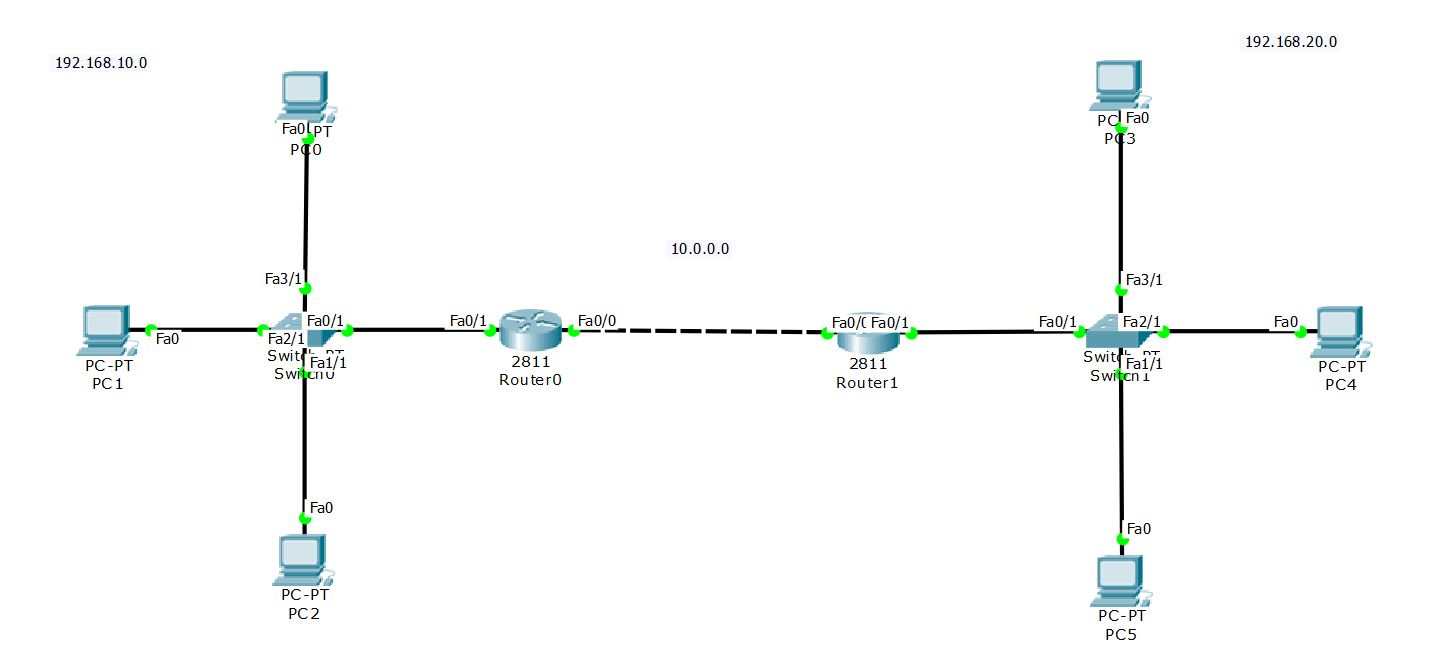
\includegraphics[width=\linewidth]{images/07.routing-sicurezza/vpn/01.jpg}
\end{center}

Per implementare la VPN site-to-site abbiamo creato questa rete come esempio, e, dopo aver posizionato e configurato i vari dispositivi sarà necessario inserire il codice, che andremo a spiegare, all’interno di uno dei router (prenderemo come esempio quello di sinistra), che è composto da poche e semplici linee:

Inizialmente, entrati nella CLI del router, si effettuerà la configurazione del RIP, un protocollo di routing che prevede l'invio dell'intera tabella di routing ogni 30 secondi

\begin{fcmds}{Configuration mode}
    \$ router rip\\
    \$ network 10.0.0.0\\
    \$ network 192.168.10.0
\end{fcmds}

Successivamente entreremo nell’area di configurazione dell’IKE che ci permetterà di decidere i parametri che verranno utilizzati nell’IKE, un protocollo ibrido che ci permetterà di configurare l’IPSec e di implementare dei sistemi per lo scambio di chiavi (Oakley key exhange e Skeme key exhange)

\begin{fcmds}{Configuration mode}
    \$ crypto isakmp policy 10\\
    \$ authentication pre-share\\
    \$ hash sha\\
    \$ encryption aes 256\\
    \$ group 2\\
    \$ lifetime 45200\\
    \$ exit\\
    \$ crypto isakmp key redhat address 10.0.0.2\\
    \$ crypto ipsec transform-set TSET esp-aes esp-sha-hmac
\end{fcmds}

Ora è arrivato il momento di creare un ACL per definire che tipo di traffico verrà inviato dalla VPN

\begin{fcmds}{Configuration mode}
    \$ access-list 101 permit ip 192.168.10.0 0.0.0.255 192.168.20.0 0.0.0.255
\end{fcmds}

Con il seguente codice verrà creata una crypto map basata sui parametri precedenti

\begin{fcmds}{Configuration mode}
    \$ crypto map CMAP 10 ipsec-isakmp\\
    \$ set peer 10.0.0.2\\
    \$ match address 101\\
    \$ set transform-set TSET
\end{fcmds}

Ed ora si applicherà la crypto map ad un’interfaccia del router

\begin{fcmds}{Configuration mode}
    \$ int fa0/0\\
    \$ crypto map CMAP\\
    \$ do write
\end{fcmds}

A questo punto la configurazione della nostra rete VPN per il router di sinistra è completa, per ultimare l’intera connessione con la VPN site-to-site sarà necessario ripetere gli stessi step sopraelencati, ovviamente utilizzando i parametri adeguati, ovvero quelli del router di destra.

Finita la configurazione per verificare il corretto funzionamento della nostra VPN site-to-site basterà semplicemente digitare il seguente codice nel router:

\begin{fcmds}{Priviledged mode}
    \$ show crypto isakmp sa
\end{fcmds}

Se verrà visualizzato un messaggio simile al seguente la configurazione è completa:

\begin{verbatim}
IPv4 Crypto ISAKMP SA
dst      src      state   conn-id slot status
10.0.0.2 10.0.0.1 QM_IDLE 1089    0    ACTIVE
\end{verbatim}

\subsubsection{VPN ad Accesso Remoto su Cisco Packet Tracer}
\begin{center}
    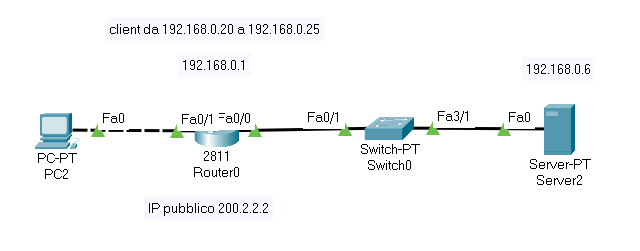
\includegraphics[width=\linewidth]{images/07.routing-sicurezza/vpn/02.png}
\end{center}

Ora invece abbiamo un esempio che riguarda le VPN ad accesso remoto, e, come in precedenza, dopo aver posizionato e configurato i vari dispositivi sarà necessario inserire il codice, che andremo a spiegare di seguito: 

Per prima cosa abilitiamo il servizio “aaa new-model", seguito da X-Auth per effettuare l’autenticazione degli utenti e del gruppo

\begin{fcmds}{Configuration mode}
    \$ aaa new-model\\
    \$ aaa authentication login default local\\
    \$ aaa authentication login vpn\_xauth\_ml\_1 local\\
    \$ aaa authentication login sslvpn local\\
    \$ aaa authorization group1 local\\
    \$ aaa session-id common
\end{fcmds}

Successivamente creiamo degli account che verranno poi messi a disposizione agli utenti remoti. Questa operazione è necessaria al fine di garantire l’inserimento di queste due informazioni ogni volta che l’utente proverà a connettersi a questa VPN

\begin{fcmds}{Configuration mode}
    \$ crypto isakmp policy 1\\
    \$ encr 3des\\
    \$ authentication pre-share\\
    \$ group 2\\
    \$ crypto isakmp policy 2\\
    \$ encr 3des\\
    \$ hash md5\\
    \$ authentcation pre-share\\
    \$ group 2
\end{fcmds}

Ora sarà necessario creare un gruppo e configurare il server DNS e gli altri parametri come richiesto. Infine gli utenti che verranno autenticati in questo gruppo otterranno un indirizzo IP dalla pool “VPN-Pool”, che offrirà indirizzi IP da 192.168.0.20 fino a 192.168.0.25

\begin{fcmds}{Configuration mode}
    \$ crypto isakmp client configuration group CCLIENT-VPN\\
    \$ key firewall.cx\\
    \$ dns 10.0.0.10\\
    \$ pool VPN-Pool\\
    \$ acl 120\\
    \$ max-users 5\\
    \$ exit\\
    \$ ip local pool VPN-Pool 192.168.0.20 192.168.0.2
\end{fcmds}

Concentriamoci adesso sulla creazione delle politiche di fase 2. Questo riguarda l’attuale autenticazione dell’encryption \& IPSec fase 2

\begin{fcmds}{Configuration mode}
    \$ crypto ipsec transform-set encrypt-method-1 esp-3des esp-sha-hmac
\end{fcmds}

La trasformazione chiamata “criptazione1” è applicata ad un profilo IPSec chiamato 'Profilo1':

\begin{fcmds}{Configuration mode}
    \$ crypto ipsec profile Profilo1\\
    \$ set transform-set criptazione1
\end{fcmds}

Ora è il momento di andare a creare una virtual-template interface, grazie a ciò i clienti della VPN otterranno un indirizzo IP remoto che fa farte della rete interna, questo ci permetterà di creare un’interfaccia non numerata, evitando l’assegnazione di IP specifici 

\begin{fcmds}{Configuration mode}
    \$ interface Virtual-Template2 type tunnel\\
    \$ ip unnumbered FastEthernet0/0\\
    \$ tunnel mode ipsec ipv4\\
    \$ tunnel protection ipsec profile Profilo1
\end{fcmds}

Dovremo poi creare l’ultimo profilo ISAKMP per connettere il gruppo utente della VPN con il template virtuale

\begin{fcmds}{Configuration mode}
    \$ crypto isakmp profile vpn-ike-profile-1\\
    \$ match identity group CCLIENT-VPN\\
    \$ client authentication list vpn\_xauth\_ml\_1\\
    \$ isakmp authorization list vpn\_group\_ml\_1\\
    \$ client configuration address respond\\
    \$ virtual-template 2
\end{fcmds}

Ed infine diamo i permessi o li neghiamo con questi due comandi:

\begin{fcmds}{Configuration mode}
    \$ access-list 120 remark ==[Cisco VPN Users]==\\
    \$ access-list 120 permit ip 10.0.0.0 0.0.0.255 192.168.50.0\\
    0.0.0.255\\
    \$ access-list 100 remark ==[Deny NAT for VPN Clients]==\\
    \$ access-list 100 deny ip 10.0.0.0 0.0.0.255 192.168.50.0 0.0.0.255
\end{fcmds}

E qui si conclude la configurazione, sicuramente più macchinosa e complicata rispetto alla VPN site-to-site, della nostra VPN ad accesso remoto.

\subsection{Tunneling}
Le informazioni che vengono trasmesse tramite Internet, o tra due dispositivi digitali, necessitano di protocolli. Tali protocolli dividono il messaggio in diverse parti (in genere due), una contenente i dati effettivi che vengono trasmessi e l'altra contenente le informazioni relative alle regole di trasmissione. Per poter stabilire una connessione, entrambe le parti coinvolte devono comprendere e utilizzare lo stesso protocollo di comunicazione. Un protocollo di tunneling include nel proprio datagramma un altro pacchetto di dati completo che utilizza un protocollo di comunicazione diverso. In sostanza, crea un tunnel tra due punti di una rete che possono trasmettere tra loro qualsiasi tipo di dato in tutta sicurezza.

In genere, questi tipi di protocolli vengono utilizzati per inviare i dati di una rete privata tramite una rete pubblica, solitamente quando si crea una VPN (Virtual Private Network), ma possono essere utilizzati anche per aumentare la sicurezza dei dati non crittografati che vengono inviati tramite una rete pubblica. Sono disponibili diversi protocolli di tunneling alquanto diffusi, ad esempio Secure Shell (SSH), Point-to-Point Tunneling (PPTP) e IPsec, ognuno dei quali è stato progettato per uno scopo specifico.

Poiché i protocolli di tunneling nascondono nel proprio datagramma un pacchetto completo, potrebbero essere utilizzati in modo improprio. Il tunneling viene spesso utilizzato per bypassare firewall non sofisticati o non configurati in modo adeguato includendo protocolli bloccati nei protocolli che il firewall lascia passare. L'uso dei protocolli di tunneling rende, inoltre, difficile il completamento di attività quali il controllo dettagliato dei pacchetti, in cui l'infrastruttura di rete analizza il datagramma alla ricerca di dati sospetti, o il filtraggio dei dati in entrata/uscita, che esegue il test di integrità funzionale degli indirizzi di destinazione dei dati per evitare potenziali attacchi. Si registrano anche casi di malware trasmessi tramite la nuova tecnologia IPv6, che deve utilizzare il tunneling per la trasmissione verso o tramite dispositivi non compatibili.

In quanto potenziale minaccia, i protocolli di tunneling devono essere utilizzati solo da professionisti IT o di rete che possano garantire che i propri sistemi siano in grado di bloccare tunnel indesiderati e siano configurati in modo da poter applicare i protocolli di sicurezza ai dati inviati tramite un tunnel noto, analogamente ai dati inviati tramite una VPN.

\subsubsection{Vantaggi}
\begin{itemize}
    \item Permette ad un protocollo straniero di essere usato su una rete che non lo supporta; (Bypassare i blocchi geografici)
    \item Protegge dall'intercettazione dei dati; (connessione sicura)
    \item Bypassare i Firewall (es. Un firewall locale potrebbe essere, per esempio, quello di un’università che non consente di collegarsi a Netflix, o un firewall nel tuo posto di lavoro, che blocca determinati siti, come ad esempio YouTube. Connettendoti tramite una VPN, il problema non esiste più.)
    \item Nasconde l’indirizzo IP;
    \item I siti visitati vedranno solo la posizione del server VPN a cui sei connesso e non la posizione reale.
\end{itemize}

\subsubsection{Svantaggi}
\begin{itemize}
    \item Connessione internet lenta, poiché essa deve venire re-instradata e criptata tramite il server.
    \item Non supportato da tutti i dispositivi
\end{itemize}

\subsubsection{Componenti Cisco}

\subsubsection*{Network devices}
Per prima cosa \textbf{verificare che i router siano compatibili} con il protocollo IPv6.\\
Due router compatibili sono: 2811 e 2911

In questo progetto utilizzeremo: 2x Router 2911, Tunnel1 e Tunnel2

\begin{center}
    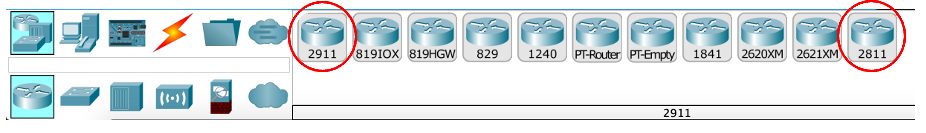
\includegraphics[width=\linewidth]{images/07.routing-sicurezza/tunneling/01.routers.png}
\end{center}

2x Switch 2950T-24 (Switch4 e Switch2)

\begin{center}
    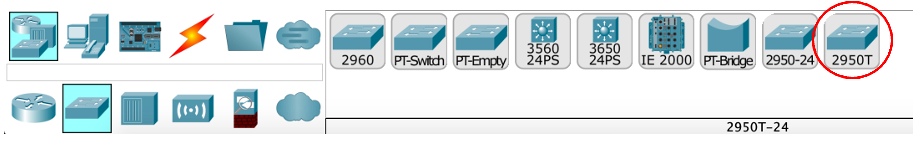
\includegraphics[width=\linewidth]{images/07.routing-sicurezza/tunneling/02.png}
\end{center}

\subsubsection*{End devices}
2x PC-PT (PC7 e PC8)

\begin{center}
    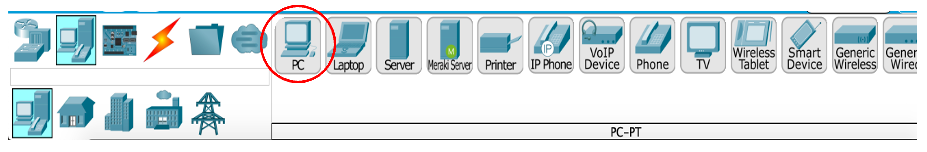
\includegraphics[width=\linewidth]{images/07.routing-sicurezza/tunneling/03.png}
\end{center}

\subsubsection*{Cavi}
Copper Cross-Over da Router0 e Router1 ai Router Tunnel1 e Tunnel2

\begin{center}
    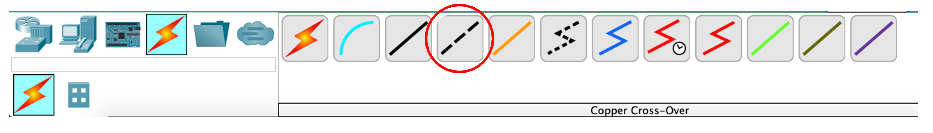
\includegraphics[width=\linewidth]{images/07.routing-sicurezza/tunneling/04.png}
\end{center}

\noindent Copper Straight-Through dai Router Tunnel1 e Tunnel2 agli Switch4 e Switch2 e dagli Switch4 e Switch2 ai PC7 e PC8

\begin{center}
    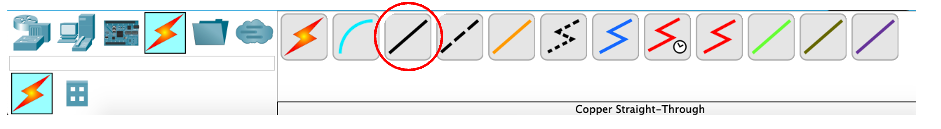
\includegraphics[width=\linewidth]{images/07.routing-sicurezza/tunneling/05.png}
\end{center}

\subsubsection*{Porte Router Tunnel1}

\begin{center}
    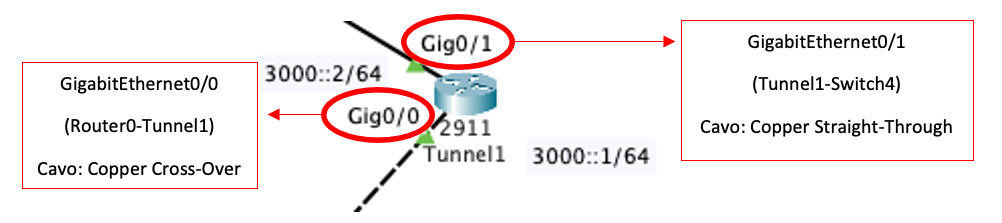
\includegraphics[width=\linewidth]{images/07.routing-sicurezza/tunneling/06.png}
\end{center}

\subsubsection*{Porte Router Tunnel2}

\begin{center}
    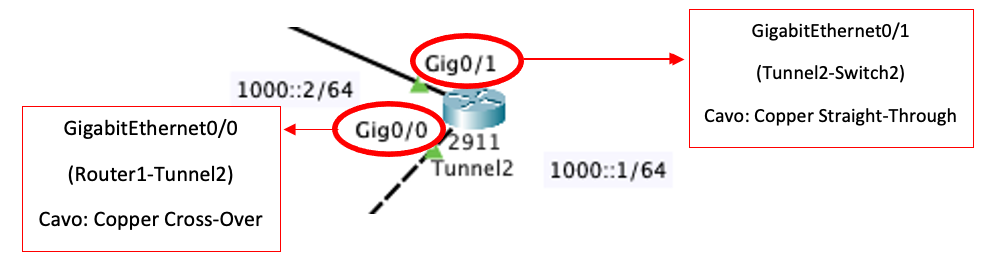
\includegraphics[width=\linewidth]{images/07.routing-sicurezza/tunneling/07.png}
\end{center}

\subsubsection*{Porte Switch4 e PC7:}

\begin{center}
    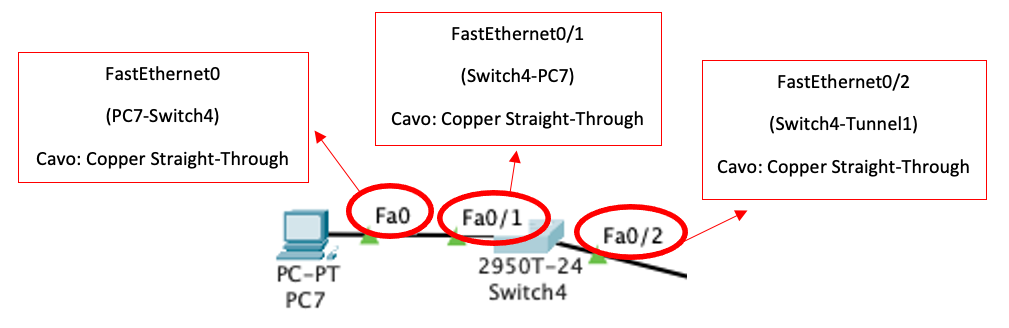
\includegraphics[width=\linewidth]{images/07.routing-sicurezza/tunneling/08.png}
\end{center}

\subsubsection*{Porte Switch2 e PC8:}

\begin{center}
    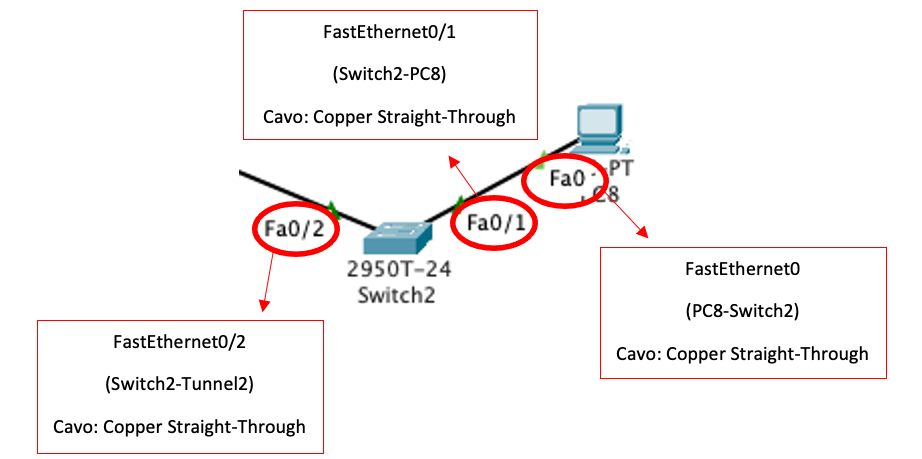
\includegraphics[width=\linewidth]{images/07.routing-sicurezza/tunneling/09.png}
\end{center}

\subsubsection{Realizzazione Tunneling}
Per poter effettuare la tecnica del tunneling sul programma Cisco Packet Tracer (in questo caso nella versione Student Version 6.2.0.0052) basterà seguire questi passaggi:

\begin{enumerate}
    \item Per prima cosa dobbiamo entrare nel Router “Tunnel2” del nostro progetto, recandoci nella sezione “CLI” di esso (Command Line Interface);\par
    \begin{center}
        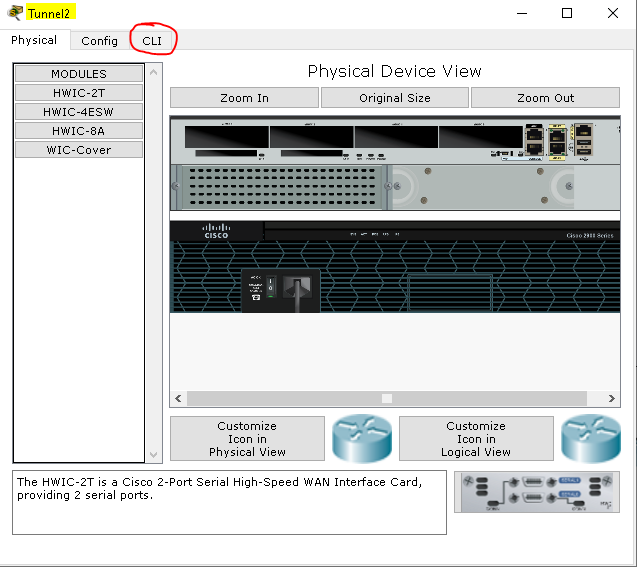
\includegraphics[width=\linewidth]{images/07.routing-sicurezza/tunneling/10.png}
    \end{center}
    \item A questo punto dovranno essere inseriti i seguenti comandi in questo ordine:\par
    \begin{fcmds}{Configuration mode}
        \$ ipv6 unicast-routing\\
        \$ interface tunnel 0\\
        \$ ipv6 address 2000::2/64\\
        \$ ipv6 rip 5info enable\\
        \$ tunnel source Gig0/0\\
        \$ tunnel destination 192.168.8.218/30\\
        \$ tunnel mode ipv6ip\\
        \$ no shutdown
    \end{fcmds}
    \item Ora che il tunnel è stato impostato, configuriamo le porte che verranno utilizzate su questo router:\par
    \begin{fcmds}{Configuration mode}
        \$ interface Gig0/1\\
        \$ ipv6 enable\\
        \$ ipv6 address 1000::1/64\\
        \$ ipv6 rip 6bone enable\\
        \$ no shutdown\\
        \$ exit\\
        \$ interface Gig0/0\\
        \$ ip address 192.168.8.214 255.255.255.252\\
        \$ no shutdown
    \end{fcmds}
    \item Configuriamo ora l’altro router (Tunnel1) incluso nel tunnel che stiamo creando;
    \item Ci rechiamo dunque anche in esso nell’interfaccia “CLI” e inseriamo i seguenti comandi:\par
    \begin{fcmds}{Configuration mode}
        \$ ipv6 unicast-routing\\
        \$ interface tunnel 0\\
        \$ ipv6 address 2000::1/64\\
        \$ ipv6 rip 6bone enable\\
        \$ tunnel source Gig0/0\\
        \$ tunnel destination 192.168.8.214/30\\
        \$ tunnel mode ipv6ip\\
        \$ no shutdown\\
        \$ interface Gig0/1\\
        \$ ipv6 enable\\
        \$ ipv6 address 3000::1/64\\
        \$ ipv6 rip 5info enable\\
        \$ no shutdown
    \end{fcmds}
    \item A questo punto abbiamo bisogno di effettuare l’Ip Route nei due router per rendergli possibile l’instradamento delle informazioni attraverso il tunnel che stiamo creando;
    \item Accediamo dunque al router “Tunneling1” e sempre nella sezione “CLI” digitiamo I seguenti comandi:\par
    \begin{fcmds}{Configuration mode}
        \$ ip route 192.168.8.212 255.255.255.252 2000::2/64
    \end{fcmds}
    \item Facciamo la stessa cosa con il router “Tunneling2”:\par
    \begin{fcmds}{Configuration mode}
        \$ ip route 192.168.8.216 255.255.255.252 2000::1/64
    \end{fcmds}
    \item Ora avremmo così creato la seguente topologia:\par
    \begin{center}
        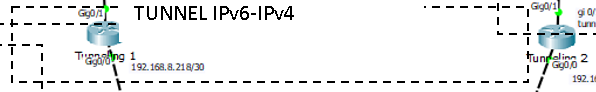
\includegraphics[width=\linewidth]{images/07.routing-sicurezza/tunneling/11.png}
    \end{center}
\end{enumerate}
